\documentclass[conference]{IEEEtran}
\usepackage[T1]{fontenc}
\usepackage{amsmath,amssymb,graphicx,booktabs,array}
\usepackage{algorithm,algpseudocode}
\usepackage[hidelinks]{hyperref}
\setcounter{topnumber}{3}
\setcounter{bottomnumber}{2}
\setcounter{totalnumber}{5}
\renewcommand{\topfraction}{0.92}
\renewcommand{\bottomfraction}{0.85}
\renewcommand{\textfraction}{0.08}
\renewcommand{\dbltopfraction}{0.92}
\begin{document}

\title{Camera-Motion Compensation for DeepSORT:\\Benefits and Limitations Across Camera Motions}
\author{\IEEEauthorblockN{Omar Hussain and Zayed Mohammed}
\IEEEauthorblockA{Department of Electrical, Computer and Biomedical Engineering\\
College of Engineering, Abu Dhabi University, Abu Dhabi, United Arab Emirates}}
\maketitle

\begin{abstract}
A person tracker must recognise the same person across video frames. When the camera moves, this task becomes harder because people shift in the image even when they are standing still. We test whether camera-motion compensation (CMC) helps DeepSORT keep identities consistent. Each comparison uses the same person detections, so only the compensation step changes. We evaluate real pedestrian and sports videos, simulated camera movements and skipped frames. On moving MOT17 videos, CMC improved Higher Order Tracking Accuracy (HOTA) by 0.48 points (95\% interval 0.18--0.78), with negligible changes on fixed-camera videos. The gain was larger during fast simulated pans, but was not consistent on independent forward-moving footage. Adjusting the tracker's time step also reduced the apparent benefit of CMC when frames were skipped. Simulated safety-equipment reporting showed fewer repeated alerts in some conditions, without clear improvement in assigning observations to the correct person. These results show where CMC can help and why it should be tested with the intended camera and tracker settings.
\end{abstract}

\begin{IEEEkeywords}
multi-object tracking, camera-motion compensation, DeepSORT, camera rotation, PPE monitoring
\end{IEEEkeywords}

\section{Introduction}
Consider a camera monitoring whether workers wear helmets and safety vests. Detecting a helmet in one image is not enough: the system must also know which worker it belongs to and whether that worker has already been recorded. A tracker gives each person an identity number and tries to retain it throughout the video. An identity change can lead to a repeated alert or an observation assigned to the wrong worker~\cite{lee2023ppe,wang2019hazards}.

The capstone that motivated this study combined YOLOv8 object detection with DeepSORT person tracking~\cite{qamhieh2025capstone}. It assigned an item of personal protective equipment (PPE) to a worker when more than 80\% of the item's box lay inside the worker's box. The system was tested with fixed cameras, but tracking accuracy under camera motion was not measured.

DeepSORT predicts where a person will appear next, then matches the prediction to a new detection~\cite{wojke2017deepsort}. Camera motion can make this prediction wrong. For example, a pan may shift everyone 10 pixels left even if nobody walks. CMC estimates that shared shift and moves the predictions before matching. It does not change which people the detector finds.

We ask when CMC improves DeepSORT, how much computation it adds, and whether its benefit changes when frames are skipped. We keep the original tracker so that compensation can be studied separately. PPE monitoring is the motivation, but the experiments use public pedestrian and sports videos rather than workers wearing PPE.

\section{Related Work}
SORT predicts object motion with a Kalman filter and matches boxes between frames~\cite{bewley2016sort,kalman1960}. DeepSORT also compares visual appearance, helping it distinguish nearby people~\cite{wojke2017deepsort}. ByteTrack uses low-confidence detections~\cite{zhang2022bytetrack}, while OC-SORT changes motion estimation after a person has been hidden from view~\cite{cao2023ocsort}.

BoT-SORT and StrongSORT already include CMC, but also change other tracking components~\cite{aharon2022botsort,du2023strongsort}. BoT-SORT estimates motion from tracked image points; StrongSORT uses image alignment. Their reported CMC gains come from different pipelines and cannot be compared directly with ours. Virtual pan--tilt--zoom (PTZ) cameras support repeatable camera-motion tests~\cite{chen2015ptz}; SportsMOT provides real footage from cameras that pan and zoom~\cite{cui2023sportsmot}. We use controlled transformations and real footage because neither alone captures all deployment conditions.

\section{Tracking Method}
\subsection{A Controlled Comparison}
A detector draws a box around each person in a frame. DeepSORT then links boxes over time using predicted motion and an appearance feature vector describing how each person looks. Our \emph{baseline} is DeepSORT without CMC. The compensated version uses the same detections and features, saved in advance for each video and detector. This prevents changes in detection from being mistaken for a CMC improvement. No model was trained.

We used pretrained YOLOv8n~\cite{jocher2023yolov8}, with 640-pixel input, person confidence 0.25 and non-maximum suppression IoU 0.8. IoU measures box overlap as intersection area divided by union area. DeepSORT used the \texttt{mars-small128} appearance network with cosine-distance limit 0.2, 100 stored appearance features, IoU-distance limit 0.7, maximum age 30 processed frames and three detections to confirm a track.

\subsection{Estimating Camera Motion}
We tested four ways to estimate how the background moves between consecutive frames.

\emph{Similarity CMC} tracks background points and fits one transformation allowing translation, rotation and uniform scaling. Person boxes are masked so that walking people do not dominate the estimate. Shi--Tomasi corner selection~\cite{shi1994good} and Lucas--Kanade optical flow~\cite{lucas1981iterative} provide point matches. \mbox{Random sample consensus (RANSAC)}~\cite{fischler1981ransac} selects the transformation supported by a sufficiently large group of matching points.

Estimation used half-resolution grayscale images, at most 1,000 corners (quality 0.01, spacing 8 pixels, block size 3), and an LK window of $21\times21$, maximum pyramid level 3, with a 30-iteration or 0.01-error stop. OpenCV's partial-affine fitting function used a 3-pixel full-resolution threshold, 2,000 maximum iterations and confidence 0.99. It returned no compensation if fewer than 30 points were tracked, fitting failed or fewer than half the points agreed. Parameters were fixed before MOT17 evaluation.

\emph{Translation-only} uses the median point displacement, with the same minimum point count and agreement threshold. It cannot represent rotation or scale changes.

\emph{Enhanced correlation coefficient (ECC) alignment}~\cite{evangelidis2008ecc} compares image intensities rather than tracked points. We fitted rotation and translation to unmasked grayscale images at 10\% resolution, using 100 maximum iterations, tolerance $10^{-5}$ and Gaussian-filter size 1. Translation was rescaled to the original image; failure returned no compensation.

\emph{Hybrid CMC} uses the similarity estimate when its checks pass and ECC otherwise (Algorithm~\ref{alg:hybrid}). The rule was developed on MOT17 results, then fixed before independent testing. Its MOT17 comparisons are therefore exploratory.

\begin{algorithm}[t]
\caption{Hybrid camera-motion estimation (exploratory)}\label{alg:hybrid}
\footnotesize
\begin{algorithmic}[1]
\State Track background corners between the two frames using LK
\If{at least 30 points remain}
  \State Fit a similarity transform by RANSAC (3-pixel threshold)
  \If{a transform exists and the inlier ratio is at least 0.5}
    \State \Return similarity transform
  \EndIf
\EndIf
\State Attempt Euclidean ECC alignment at 10\% resolution
\If{alignment returns without failure}
  \State \Return ECC transform with translation rescaled
\EndIf
\State \Return identity transform
\end{algorithmic}
\end{algorithm}

\subsection{Applying Compensation}
CMC is applied after DeepSORT predicts each track and before it matches tracks to detections. In the 10-pixel example, every predicted centre is moved 10 pixels left. A similarity transformation also rotates or scales the predictions when needed.

Let $\mathbf{p}$ be a predicted centre, $M=sR$ a rotation with scale $s$, and $\mathbf{t}$ a translation. Following BoT-SORT~\cite{aharon2022botsort}, we update
\begin{equation}
\mathbf{p}'=M\mathbf{p}+\mathbf{t},\qquad P'=TP T^\top.
\end{equation}
Here $P$ is the Kalman filter's uncertainty matrix and $T$ applies the same coordinate change to the state. For DeepSORT's state $(u,v,\gamma,h,\dot u,\dot v,\dot\gamma,\dot h)$, $T=\operatorname{blockdiag}(M,1,s,M,1,s)$. Height and its rate of change scale by $s$; aspect ratio stays unchanged. Updating uncertainty avoids mixing the old and new coordinates.

\subsection{Handling Skipped Frames}
Processing every $k$-th frame creates a larger time gap. The default tracker still makes one prediction per processed frame ($\Delta t=1$), and its maximum age of 30 spans roughly $30k$ original frames. We call this the \emph{default-step} setting.

The \emph{time-aware} setting uses $\Delta t=k$, multiplies process-noise covariance by $k$ and sets maximum age to $\lceil30/k\rceil$. This keeps track lifetime close to 30 original frames and allows greater uncertainty across a gap. Linear noise scaling is a sensitivity choice, not a uniquely correct model. Confirmation length and appearance memory remain unchanged. Baseline and CMC share each setting; separate checks changed only age or the combined time-step/noise settings.

\section{Experimental Design}
\subsection{Real Footage and Detection Sources}
MOT17~\cite{milan2016mot16} provides videos in which people are manually boxed and assigned identity numbers. Its seven training videos contain 5,316 frames: three fixed-camera sequences (02, 04, 09) and four moving-camera sequences (05, 10, 11, 13). We used YOLOv8n and public Faster R-CNN (FRCNN) detections, keeping FRCNN confidence $\geq0.25$ without further suppression. Frame-skipping tests retained every 2nd, 3rd or 6th frame, with detections and reference labels adjusted consistently.

To test different footage, we used three moving-camera MOT15 sequences~\cite{lealtaixe2015mot15}: ETH-Bahnhof, ETH-Sunnyday and KITTI-13, totalling 1,694 frames at 10--14~fps. Four MOT15 videos duplicating MOT17 were excluded. We used YOLOv8n and the public aggregate channel features (ACF) detections, the latter without an extra threshold. The rules were fixed before these runs.

SportsMOT~\cite{cui2023sportsmot} supplied the lowest-numbered validation clip from each of 13 source videos: 8,074 frames at 25~fps. The selection was recorded before evaluation. These tests used YOLOv8n at full frame rate. Broadcast pans and zooms provide real camera motion, but athletes differ from construction workers.

\subsection{Simulated Camera Motion}
\emph{Moving crops.} We moved a window covering 80\% of each image dimension over the three fixed-camera MOT17 videos. Each produced eight variants: still, back-and-forth pans at 2, 5, 10 and 20 pixels/frame, and random position changes with standard deviation 2, 5 or 10 pixels. This gives known image motion while retaining real people and backgrounds. Detection was rerun once per variant and shared across tracking conditions.

Reference boxes were shifted by the crop offset. Fully outside boxes were removed; visibility was multiplied by the in-window area fraction. Pedestrians less than 25\% inside were marked as distractors, while remaining boxes stayed unclipped. An \emph{oracle} control applied the exact image shift, allowing us to separate motion-estimation error from the benefit of compensation.

\emph{Virtual camera rotation.} We also transformed frames to imitate pan sweeps and angular sway. A homography, an image-coordinate mapping, represented rotation about the camera's optical centre. The reference image used a 60$^\circ$ horizontal field of view and focal length 1,662.8 pixels at width 1,920, scaled with width. The output covered two-thirds of each dimension. Focal length stayed fixed, so these PTZ-style tests did not include zoom.

Sweeps moved between $\pm8^\circ$ at 5--40$^\circ$/s with one-second pauses. Sway used 0.8~Hz pan, 1.1~Hz tilt, pan amplitude 0.1--0.5$^\circ$ and tilt amplitude 0.6 times pan. Random pan bumps used twice the amplitude, 3~Hz oscillation, 0.5~s decay and Poisson rate 0.25/s (seed 0). Translational pole motion was not simulated.

Sources were the three fixed MOT17 videos and four non-duplicate fixed MOT15 videos: PETS09-S2L1, TUD-Stadtmitte, TUD-Campus and KITTI-17 (7--25~fps). MOT15 used still, 10--40$^\circ$/s sweeps and 0.5$^\circ$ sway; MOT17 also used milder levels. Reference box corners were transformed and enclosed in axis-aligned boxes, using the crop visibility rule.

YOLOv8n was rerun on transformed frames. For the three MOT17 scenes, FRCNN boxes were instead transformed, clipped and retained if at least 50\% inside; appearance features were recomputed. This tests another detection source, not FRCNN inference on distorted images.

For rotations, the oracle fitted a similarity to the known inter-frame homography on a $9\times9$ grid using OpenCV's least-median-of-squares option. It is an approximation, unlike the exact crop-shift oracle. A separate simulation estimated compensation from camera-angle readings with noise of 0, 0.1 or 0.3$^\circ$ and delays of 0, 1 or 3 frames. No physical sensors were used.

\subsection{Simulated PPE Reporting}
We assigned each labelled person a fixed simulated PPE status, with a 20\% probability of non-compliance and a deterministic sequence-based seed. Person boxes were matched to tracker boxes by Hungarian assignment at IoU $>0.5$. A track's owner was defined retrospectively as the person it matched most often. This tests identity-dependent reporting, not PPE detection or the capstone's 80\% containment rule.

We counted observations assigned to the wrong owner and observations with a PPE status different from the owner's. Both exclude unmatched observations. We also counted tracks owned by non-compliant people per matched non-compliant person. Multiple tracks can produce repeated alerts, but misses and merges can also lower this ratio. Its denominator can differ between conditions. We repeated status assignment 1,000 times to show sensitivity to which people were labelled non-compliant; displayed ratios use one fixed assignment.

\subsection{How Performance Was Measured}
TrackEval~\cite{luiten2020trackeval} compared tracker outputs with the manual labels. Our main score, HOTA, balances finding people correctly with linking their identities across frames~\cite{luiten2021hota}. IDF1 measures identity consistency~\cite{ristani2016idf1}, and IDSW counts identity changes. HOTA and IDF1 range from 0 to 100, with higher values better; fewer switches are better. AssA isolates association accuracy. Multiple object tracking accuracy (MOTA) and fragmentation~\cite{bernardin2008clear} were supporting measures.

Every reported change is CMC minus its matching baseline, in score points or switch counts. Group results use TrackEval's combined calculation. For example, a change of $+0.48$ means a score rose by 0.48 points, not by 48\%.

We estimated 95\% intervals by drawing 1,000 paired samples of 60 consecutive processed-frame blocks, wrapping at sequence ends~\cite{kunsch1989bootstrap} (seed 2026). The same frame samples were used for labels and saved outputs, then scores were recomputed without rerunning tracking. These intervals describe variation within the tested footage, not new scenes; block joins and different frame rates also affect them. We additionally removed one video at a time and recomputed combined scores. A one-sided sign test assumed equal chances of positive and negative changes. Secondary intervals are descriptive, without multiple-comparison correction.

\subsection{Implementation and Timing}
Baseline and similarity CMC were repeated on two CPUs: two Xeon cores at 2.10~GHz (Python 3.13, OpenCV 5.0, NumPy 2.5) and four ARM64 cores (Python 3.10.12, OpenCV 5.0.0, NumPy 2.2.6, ONNX Runtime 1.23.2). Model files were checked by SHA-256. Tables use ARM64 results; expanded experiments were not all repeated across machines. Xeon point-based timing excludes decoding, grayscale conversion and resizing. ARM64 ECC timing includes grayscale conversion and resizing, so the timings do not establish which estimator is faster.

\section{Results}
\subsection{MOT17 and Translating Crops}
On fixed-camera MOT17 videos, changes were negligible: at most 0.02 HOTA and 0.05 IDF1 points. On moving videos, similarity CMC improved HOTA by 0.48 with YOLOv8n (Table~\ref{tab:mot17}). However, the IDF1 interval crossed zero, meaning these data did not clearly establish an identity-score improvement for that detector.

\begin{table}[t]
\caption{Moving MOT17 videos at full rate, similarity CMC. Base is the score without CMC; changes are score points or switch counts. The 95\% intervals refer to the change. FRCNN: Faster R-CNN; AssA: association accuracy; IDSW: identity switches.}
\label{tab:mot17}
\centering\footnotesize
\setlength{\tabcolsep}{3.5pt}
\begin{tabular}{@{}lrrrr@{}}
\toprule
 & \multicolumn{2}{c}{YOLOv8n} & \multicolumn{2}{c}{FRCNN}\\
\cmidrule(lr){2-3}\cmidrule(l){4-5}
Measure & Base & Change & Base & Change\\
\midrule
HOTA & 37.48 & +0.48 & 47.86 & +0.45\\
95\% interval & \multicolumn{2}{c}{[0.18, 0.78]} & \multicolumn{2}{c}{[0.08, 0.83]}\\
IDF1 & 45.29 & +0.25 & 56.32 & +0.92\\
95\% interval & \multicolumn{2}{c}{[$-$0.27, 0.87]} & \multicolumn{2}{c}{[0.04, 1.31]}\\
AssA & 41.22 & +0.69 & 50.07 & +0.48\\
IDSW & 441 & $-$25 & 297 & $-$11\\
\bottomrule
\end{tabular}
\end{table}

All four moving videos gained HOTA. The sign-test result was $p=0.0625$, the smallest possible value with four positive results. Removing any one video kept gains at 0.40--0.55 with YOLOv8n and 0.28--0.57 with FRCNN. Thus one video did not account for the combined improvement. Fig.~\ref{fig:real} shows an example of an identity retained by CMC.

Fast moving crops gave larger gains. At 20 pixels/frame, IDF1 rose from 27.8 to 40.2 and switches fell from 987 to 371 in ARM64. The two machines gave gains of 12--14 IDF1 points, although smaller-motion effects changed direction. Estimated compensation stayed within 0.47 IDF1 points of the exact crop oracle, suggesting motion-estimation error was not the main limitation in these tests.

\begin{figure*}[t]
\centering
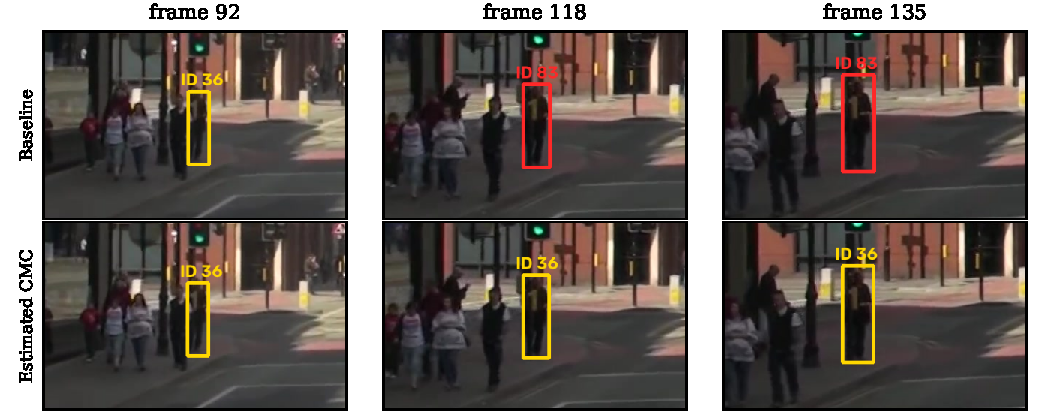
\includegraphics[width=0.70\textwidth]{figures/fig_real13.pdf}
\caption{MOT17-13, real moving camera, YOLOv8n at full rate: frames 92, 118 and 135. Only the track matched to one pedestrian is drawn. The baseline replaces identity 36 with 83 at frame 102; similarity CMC retains 36. This selected example illustrates a mechanism rather than the average effect. Frames from MOT17~\cite{milan2016mot16} (CC BY-NC-SA 3.0); overlays by the authors.}
\label{fig:real}
\end{figure*}

\subsection{Simulated Angular Motion}
Faster simulated sweeps generally gave larger gains on MOT17 (Table~\ref{tab:ptz}). At 40$^\circ$/s, similarity CMC gained 5.38 HOTA with YOLOv8n and 8.72 with mapped FRCNN. Switches fell from 761 to 424 and from 773 to 249, reductions of 44\% and 68\%.

\begin{table}[t]
\caption{Simulated sweeps: combined HOTA change with similarity CMC. Intervals describe the change. MOT15 contains four scenes; each MOT17 group contains three. FRCNN boxes were geometrically mapped. Lower frame rates give larger motion per frame at the same sweep speed.}
\label{tab:ptz}
\centering\footnotesize\setlength{\tabcolsep}{4pt}
\begin{tabular}{@{}lrrrr@{}}
\toprule
Scene group / detector & Speed & Without & Gain & 95\% interval\\
 & ($^\circ$/s) & CMC & & \\
\midrule
MOT17 / YOLOv8n & 20 & 26.9 & +1.80 & [1.2, 3.1]\\
 & 40 & 23.1 & +5.38 & [4.3, 7.0]\\
MOT17 / FRCNN & 20 & 32.7 & +2.33 & [1.9, 3.3]\\
 & 40 & 25.6 & +8.72 & [7.2, 10.7]\\
MOT15 / YOLOv8n & 10 & 31.3 & +18.67 & [15.1, 21.7]\\
 & 20 & 26.7 & +22.22 & [19.9, 25.2]\\
 & 40 & 26.1 & +5.75 & [5.0, 8.9]\\
\bottomrule
\end{tabular}
\end{table}

On MOT17 rotations, estimated and oracle compensation differed by at most 0.6 HOTA and similarity estimation never failed its checks. The lower-frame-rate MOT15 scenes gained 22.22 at 20$^\circ$/s, but only 5.75 at 40$^\circ$/s compared with 22.78 from the oracle. Here, knowing the motion helped much more than estimating it. Scene content also differs, so frame rate alone cannot explain the difference. Angular sway of 0.5$^\circ$ gained 0.83 and 1.58 HOTA on MOT17, while the MOT15 interval crossed zero; milder sway changes were small.

\subsection{Real Sports Footage and Independent Pedestrians}
Real sports footage gained 1.43 HOTA and 1.46 IDF1 with similarity CMC (Table~\ref{tab:sports}). Eight of 13 clips improved, while ECC improved ten. Switches increased by 58, showing that a higher overall score does not necessarily mean fewer identity changes. The exploratory hybrid had the largest combined gain, but no interval was computed for it.

\begin{table}[t]
\caption{SportsMOT, 13 clips, YOLOv8n. Baseline HOTA 27.6, IDF1 27.5 and 3,286 switches. Changes are relative to the same baseline. The similarity HOTA interval is [0.55, 1.81] and IDF1 interval [0.20, 2.18].}
\label{tab:sports}
\centering\footnotesize\setlength{\tabcolsep}{6pt}
\begin{tabular}{@{}lrrr@{}}
\toprule
Method & HOTA change & IDF1 change & Switch change\\
\midrule
Similarity & +1.43 & +1.46 & +58\\
Translation & +0.70 & +0.50 & +48\\
ECC & +1.01 & +0.81 & $-$8\\
Hybrid (exploratory) & +1.65 & +1.87 & +10\\
\bottomrule
\end{tabular}
\end{table}

The independent MOT15 pedestrian videos did not show a consistent benefit (Table~\ref{tab:m15}). With YOLOv8n, HOTA fell by 0.63 and IDF1 by 1.61; the IDF1 interval [$-$2.84, $-$0.10] excluded zero. Losses were mainly on forward-moving ETH footage. KITTI-13 changed little, with no compensation applied on 63\% of frames because point-based estimation failed its checks. With ACF detections, the IDF1 interval [$-$2.34, 1.15] crossed zero. ECC and hybrid also lost HOTA with full-rate YOLOv8n ($-0.67$ and $-0.68$).

\begin{table}[t]
\caption{Independent moving-camera videos at full frame rate, similarity CMC. Changes are relative to no CMC. ACF is the public MOT15 detector; other rows use YOLOv8n.}
\label{tab:m15}
\centering\footnotesize\setlength{\tabcolsep}{5pt}
\begin{tabular}{@{}lrrr@{}}
\toprule
Video / detection source & Baseline HOTA & HOTA change & IDF1 change\\
\midrule
ETH-Bahnhof & 33.4 & $-$0.47 & $-$1.19\\
ETH-Sunnyday & 55.2 & $-$1.43 & $-$3.85\\
KITTI-13 & 33.9 & +0.47 & +0.16\\
Combined / YOLOv8n & 38.4 & $-$0.63 & $-$1.61\\
Combined / ACF & 34.7 & $-$0.10 & $-$0.48\\
\bottomrule
\end{tabular}
\end{table}

\subsection{Frame Skipping and Tracker Configuration}
Allowing for the larger time gap improved the baseline substantially (Table~\ref{tab:stride}). When processing every sixth frame, its HOTA rose from 29.9 to 35.0 with YOLOv8n and from 31.6 to 40.3 with FRCNN. The additional ECC gain then fell from 5.43 to 0.69 (interval [$-$0.27, 1.77]) and from 10.12 to 2.74 ([1.62, 3.91]). Changing track lifetime alone retained the large gains. The combined time-step and noise changes therefore mattered, although their separate effects were not established.

\begin{table}[t]
\caption{Frame skipping on moving MOT17 videos: HOTA without CMC and additional gain from ECC. The time-aware tracker accounts for the larger gap. $k$ means every $k$-th frame is processed.}
\label{tab:stride}
\centering\footnotesize
\setlength{\tabcolsep}{4pt}
\begin{tabular}{@{}lrrrrr@{}}
\toprule
 & & \multicolumn{2}{c}{Default step} & \multicolumn{2}{c}{Time-aware}\\
\cmidrule(lr){3-4}\cmidrule(l){5-6}
Detector & $k$ & Base & ECC gain & Base & ECC gain\\
\midrule
YOLOv8n & 2 & 36.9 & +1.37 & 37.6 & +0.58\\
 & 3 & 35.3 & +3.97 & 38.7 & +0.94\\
 & 6 & 29.9 & +5.43 & 35.0 & +0.69\\
FRCNN & 2 & 45.5 & +3.07 & 46.8 & +1.23\\
 & 3 & 39.9 & +7.03 & 45.2 & +2.30\\
 & 6 & 31.6 & +10.12 & 40.3 & +2.74\\
\bottomrule
\end{tabular}
\end{table}

\subsection{Simulated Angle Readings}
Camera-angle readings could provide compensation without estimating motion from images. With noiseless readings, a 40$^\circ$/s sweep gained 5.32 HOTA with no delay, 3.32 with one frame of delay and lost 0.98 with three frames. Image-based similarity gained 5.38. At 20$^\circ$/s, the corresponding angle-reading gains were 2.28, 1.74 and 0.66. Without delay, noise of 0.1$^\circ$ retained gains of 2.31 and 5.22 for the two speeds; 0.3$^\circ$ retained 0.95 and 3.85. These simulated results show latency sensitivity, not a strict requirement for zero delay.

\subsection{Simulated PPE Outcomes}
CMC reduced repeated-report ratios in some fast-motion tests, but did not consistently improve assignment to the correct person (Table~\ref{tab:ppe}). At a 40$^\circ$/s sweep, reports per matched non-compliant person fell from 6.05 to 3.30. The number of matched people also changed from 19 to 20, so the ratio reflects both track counts and coverage. Wrong-owner observations fell from 9.1\% to 7.7\% there, but rose from 7.7\% to 8.1\% on full-rate moving MOT17 footage.

\begin{table}[t]
\caption{Simulated repeated reports with similarity CMC. B/C: baseline/CMC matched non-compliant people. Reports are tracks per matched non-compliant person, not actual detected PPE violations.}
\label{tab:ppe}
\centering\footnotesize\setlength{\tabcolsep}{6pt}
\begin{tabular}{@{}lrrr@{}}
\toprule
Condition & People & Reports & Reports\\
 & (B/C) & without CMC & with CMC\\
\midrule
MOT17 moving, full rate & 60/60 & 1.78 & 1.65\\
MOT17, every sixth frame & 25/29 & 1.80 & 1.45\\
\quad Time-aware setting & 27/30 & 1.19 & 1.10\\
MOT15 moving, full rate & 39/39 & 0.95 & 0.97\\
Crop pan 20 pixels/frame & 24/23 & 5.50 & 1.70\\
Sweep 20$^\circ$/s & 14/15 & 4.14 & 3.13\\
Sweep 40$^\circ$/s & 19/20 & 6.05 & 3.30\\
Sway 0.5$^\circ$ & 29/28 & 2.86 & 2.71\\
\bottomrule
\end{tabular}
\end{table}

Across random status redraws, the central 95\% ranges of report-ratio changes were [$-$2.35, $-$0.22] for the fast sweep and [$-$5.43, $-$1.62] for the fast crop pan. These ranges concern different simulated status assignments; they are not intervals centred on the fixed-assignment differences of $-2.75$ and $-3.80$. Merged tracks can also reduce report counts, so fewer reports alone do not prove better monitoring.

\subsection{Repeatability and Processing Cost}
The two machines differed by at most 0.07 HOTA and 0.10 IDF1 on combined real videos, but by up to 4.2 IDF1 on synthetic footage. Repeated runs from saved inputs on one machine were identical. The original environment was unavailable for a stage-by-stage comparison, so the source of cross-machine differences remains unresolved.

On Xeon, point-based estimation took a median 11.40~ms per 1080p frame (interquartile range 10.54--12.54) and 2.01~ms at $640\times480$ (1.75--2.29), excluding preprocessing. Tracker updates took 2.92~ms without and 3.20~ms with state warping. Detection and appearance encoding took 91.8 and 82.4~ms at 1080p, as medians over sequence medians. Adding component medians suggests about 7\% overhead, rather than measuring end-to-end overhead directly. ARM64 ECC took 2--4~ms including preprocessing; different hardware and timing boundaries prevent a speed comparison.

\section{Discussion}
CMC helps when camera motion moves people away from otherwise useful predictions. This explains why fast simulated pans improved substantially while fixed-camera results barely changed. The independent tests show that the same correction does not help every moving camera. When a camera travels forward, nearby and distant people can move differently in the image. A single shared transformation may then be unsuitable. This is a plausible explanation for the ETH losses, but depth and camera direction were not independently controlled.

The frame-skipping result has a practical implication: first ensure the tracker accounts for the larger time gap. Otherwise CMC may appear to solve a problem partly caused by the prediction settings. After the time-aware change, ECC still helped FRCNN at every sixth frame, while the YOLOv8n HOTA interval crossed zero.

\emph{Limits.} Simulated rotation excludes blur, rolling shutter, zoom and translational sway; its oracle is approximate. FRCNN boxes were mapped geometrically, and real sports footage shows athletes. Only seven distinct moving pedestrian videos were tested. Resampling frames cannot establish performance on new scenes. Expanded experiments were measured once, moderate synthetic effects varied between machines, and hybrid comparisons remain exploratory. We did not compare complete modern trackers.

The PPE simulation shows a possible effect of track fragmentation, not validated worker safety performance. A follow-up should use consented worker footage, real PPE annotations, a common population for report comparisons, and measures of missed observations as well as wrong assignments.

\section{Conclusion}
CMC gave small gains on moving MOT17 videos and larger gains under fast simulated pans. Real sports footage improved modestly, while independent forward-moving footage did not show consistent benefit. Frame-skipping gains depended on prediction settings. Fewer simulated repeated reports did not establish better PPE assignment. CMC is therefore worth evaluating for the intended camera motion and processing rate, rather than assuming that it improves every moving-camera tracker.

\section*{Acknowledgment}
This study builds on the capstone work of Lana Maher Qamhieh and Maha Mohamed Abueida~\cite{qamhieh2025capstone} and was conducted under the supervision of Dr.~Anas Altarabsheh and Prof.~Mohammed Ghazal.

\section*{Declaration}
This study used public MOT17, MOT15 and SportsMOT data; no new footage was collected or participants recruited. Claude (Anthropic) assisted with research, experiments and reviewing results for accuracy. Jenny AI assisted with proofreading. The authors verified the findings and take responsibility for the manuscript.

\bibliographystyle{IEEEtran}
\bibliography{refs}
\end{document}
